\chapter{Observation Design, Error Budget, and Feasibility}
\label{chap:e15}

\begin{chapteropening}
Up to this point, we have assembled the full toolbox: Chapter~\ref{chap:e11} told us how the signal-to-noise ratio of intensity interferometry scales with telescope area, photon rate, and integration time; Chapter~\ref{chap:e12} told us how much extractable information is really hidden in a dataset (Fisher information and the Cramér--Rao lower bound); Chapter~\ref{chap:e13} explained detectors, clocks, and event tables, and Chapter~\ref{chap:e14} explained how the correlator turns an event table into $g^{(2)}(\tau)$ and $|V|^2(B)$. What we must do now is \textbf{assemble these parts into one real observation}. Imagine before you a blank observing proposal form: which star will you observe? With how many telescopes, how long a baseline, how wide a filter? For how long will you expose? And in the end, to what fraction of a percent can you measure the angular diameter? This chapter is the process of filling in this form from beginning to end. At its core is a \textbf{ledger}: the photon rate gives the statistical ceiling, the correlation contrast gives the target signal, and the baseline, bandwidth, time resolution, and calibration error decide whether this signal can survive out of the noise. We will compute every step as a real number, and finally walk through a complete feasibility calculation, from one real bright star to an achievable precision.
\end{chapteropening}

\section{An observation is a ledger from parameters to data}
\label{sec:e15-ledger}

Every observation, at bottom, is for the sake of estimating a few physical numbers. The angular diameter of a star, the angular separation of a binary, the oblateness and long-axis direction of a rapid rotator, the radius of a spectral-line emitting region, the rotation of the polarization angle, the time delay between two signal paths, the height of a second-order correlation peak: these are what we really want, called the \textbf{physical parameters}, denoted $\bm\theta_{\rm phys}$. But what the instrument hands us is never these numbers; it is the \textbf{event list} of Chapter~\ref{chap:e13}: one photon per line, carrying arrival time, telescope number, wavelength, and polarization labels. The physical parameters must be \emph{inferred backwards} from these fields.

So the first thing in designing an observation is not to ask "which star do I want to look at," but to ask "do the numbers I want have supporting fields in the event table?" To do nanosecond-scale time correlation, the time-stamp precision must be compressed to the nanosecond; to give the required baseline, the position labels must be recorded accurately; to separate bands or measure polarization, the wavelength and polarization labels must not be erased at the moment of recording. Here is a principle easily overlooked yet fatal: \textbf{once information is averaged away at the recording stage, it can never be recovered afterwards}. If you store only one long-integration image from the start, then nanosecond time correlation and polarization correlation have already vanished with the averaging; whereas if you honestly store the entire event table, you can afterwards project it arbitrarily into a light curve, $g^{(2)}(\tau)$, $|V|^2(B)$, polarization angle, or multi-wavelength $u,v$ data. The event table is the "raw broth," and the image is only "one spoonful after boiling it dry."

The whole chain from parameters to data can be written as a likelihood:

\begin{equation}
  \mathcal L(\bm\theta_{\rm phys})
  =
  P\!\left(\,d \;\middle|\;
  q_{\rm inst}(\bm\theta_{\rm phys}),\;
  \bm c_{\rm cal},\;
  \bm b_{\rm sky}
  \right).
  \label{eq:e15-likelihood}
\end{equation}
\begin{formulaexplain}
$\bm\theta_{\rm phys}$: the physical parameters to be estimated (such as the angular diameter $\theta$). $d$: the observed data or its statistic. $q_{\rm inst}$: the quantity the instrument actually measures (such as $|V|^2$). $\bm c_{\rm cal}$: the calibration parameters. $\bm b_{\rm sky}$: the sky background. This formula says: the physical parameters are first "translated" by the instrument into observables, and then, together with calibration and background, determine the probability of the data appearing.
\end{formulaexplain}

Let us land each symbol. $\mathcal L$ is the likelihood, dimensionless, measuring "if the true parameters are $\bm\theta_{\rm phys}$, how probable is it to see this data $d$." $q_{\rm inst}$ is the instrument observable: it can be the squared visibility $|V|^2$ (dimensionless), the excess of the second-order correlation $g^{(2)}-1$ (dimensionless), a polarization Stokes component, or an arrival-time residual (seconds). $\bm c_{\rm cal}$ are the calibration parameters (time zero point, filter passband, detector efficiency, gain state), which are not the physical quantities we want, yet contaminate the data and must be estimated jointly or measured in advance. $\bm b_{\rm sky}$ is the skyglow, moonlight, dark counts, and host-galaxy background. When writing an observing proposal, rather than vaguely saying "we will observe this star," what is truly useful is to compute this chain all the way through: what is this star's magnitude $m_B$, how large is its estimated angular diameter $\theta$, how long is its visibility window, which $|V|^2$ data points the model prior gives, and to what fraction of a percent the error of $\theta$ can finally be pressed. The remaining sections of this chapter fill in this chain, segment by segment, with real numbers.

\section{Photon budget: from magnitude to effective photon number}
\label{sec:e15-photon-budget}

Everything begins with the photon rate. No matter how interesting a star is, if it gives you only a few photons per second, any correlation signal will drown in the noise. So the first step of a feasibility calculation is always to \textbf{translate the magnitude into photons per second}. This translation has four steps: magnitude $\to$ spectral flux density $\to$ photon flux per unit area $\to$ multiply by area and efficiency to get the effective photon rate. Let us take them one by one.

\paragraph{Step 1: magnitude to spectral flux density}

Astronomy uses the magnitude to describe brightness, with each 5 magnitudes smaller being 100 times brighter: this is a logarithmic ruler. The advantage of the AB magnitude is that it corresponds directly to the spectral flux density:

\begin{equation}
  F_\nu = 3631\,{\rm Jy}\times 10^{-0.4\,m_{\rm AB}}.
  \label{eq:e15-ab-flux}
\end{equation}
\begin{formulaexplain}
$m_{\rm AB}$: the AB magnitude (dimensionless). $F_\nu$: the spectral flux density per unit frequency. $1\,{\rm Jy}=10^{-23}\,{\rm erg\,s^{-1}\,cm^{-2}\,Hz^{-1}}$. The constant $3631\,{\rm Jy}$ is the defining flux of $m_{\rm AB}=0$. Each increase of 5 in magnitude drops $F_\nu$ by a factor of 100.
\end{formulaexplain}

Here $F_\nu$ is the spectral flux density, with dimensions of "energy / (time $\cdot$ area $\cdot$ frequency)," in CGS units ${\rm erg\,s^{-1}\,cm^{-2}\,Hz^{-1}}$; $1\,{\rm Jy}$ (jansky) $=10^{-23}$ of this unit. Take a star of $m_{\rm AB}=5$, and substituting gives
\[
  F_\nu = 3631\,{\rm Jy}\times 10^{-0.4\times5}
        = 3631\times10^{-2}\,{\rm Jy}
        = 36.3\,{\rm Jy}
        = 3.63\times10^{-22}\,{\rm erg\,s^{-1}\,cm^{-2}\,Hz^{-1}} .
\]
This is the energy this star delivers each second across each square centimetre, at each hertz of frequency. The number is very small: one square centimetre, one hertz of bandwidth, receives only $10^{-22}$ erg in one second, which reminds us that we must later gather it up with large area and wide bandwidth.

\paragraph{Step 2: energy flux to photon flux}

The detector counts not energy but numbers of photons. A photon of frequency $\nu$ carries energy $h\nu$ ($h=6.63\times10^{-27}\,{\rm erg\,s}$ is Planck's constant). Dividing the energy flux by the single-photon energy gives the number of photons per unit area, per unit time, per unit bandwidth. Multiplying by the optical bandwidth $\Delta\nu$ gives the number of photons per square centimetre per second over the whole passband. The bandwidth conversion follows the relation of Chapter~\ref{chap:e02}, $\Delta\nu\simeq c\,\Delta\lambda/\lambda^2$. Take the observing wavelength $\lambda=550\,{\rm nm}$ and passband $\Delta\lambda=10\,{\rm nm}$:
\[
  \nu=\frac{c}{\lambda}=\frac{3\times10^{10}\,{\rm cm\,s^{-1}}}{550\times10^{-7}\,{\rm cm}}
     =5.45\times10^{14}\,{\rm Hz},
  \qquad
  h\nu = 6.63\times10^{-27}\times5.45\times10^{14}
       = 3.61\times10^{-12}\,{\rm erg},
\]
\[
  \Delta\nu = \frac{c\,\Delta\lambda}{\lambda^2}
            = \frac{3\times10^{10}\times10\times10^{-7}}{(550\times10^{-7})^2}
            = 9.9\times10^{12}\,{\rm Hz}\approx10^{13}\,{\rm Hz}.
\]
Hence the photon flux per unit area
\[
  \Phi = \frac{F_\nu\,\Delta\nu}{h\nu}
       = \frac{3.63\times10^{-22}\times 9.9\times10^{12}}{3.61\times10^{-12}}
       \approx 1.0\times10^{3}\ {\rm photons\,s^{-1}\,cm^{-2}} .
\]
One square centimetre, a 10 nm passband, about a thousand photons per second: this is the raw flux \emph{arriving at the top of the atmosphere}, not yet discounted.

\paragraph{Step 3: multiply by area and efficiency to get the effective photon rate}

The photons that truly fall into the correlator must be multiplied by two more factors: the telescope's \textbf{effective collecting area} $A$, and the \textbf{total efficiency} $\eta$ from the atmosphere to photon counting. The latter folds atmospheric transmission, mirror reflectivity, filter transmission, fibre-coupling loss, and detector quantum efficiency (see Chapter~\ref{chap:e07}) all into one number, with a typical value $\eta\sim0.2$--$0.3$. Together:

\begin{equation}
  R_\gamma
  = \eta\,A\,\frac{F_\nu\,\Delta\nu}{h\nu}
  = \eta\,A\,\Phi .
  \label{eq:e15-photon-rate}
\end{equation}
\begin{formulaexplain}
$R_\gamma$: the effective photon rate (counts per second). $\eta$: the total efficiency (dimensionless, including atmosphere, mirror, filter, detector). $A$: the effective collecting area (${\rm cm^2}$). $\Phi$: the photon flux per unit area. This formula finally turns "how bright the star is" into "how many times the detector fires per second."
\end{formulaexplain}

Plug in real numbers. An imaging atmospheric Cherenkov telescope (IACT) of 12 m aperture has a collecting area $A=\pi(6\,{\rm m})^2\approx113\,{\rm m^2}=1.13\times10^6\,{\rm cm^2}$. Take $\eta=0.25$, $m_{\rm AB}=5$:
\[
  R_\gamma = 0.25\times1.13\times10^6\times1.0\times10^3
          \approx 2.8\times10^8\ {\rm s^{-1}} .
\]
About three hundred million photons per second. If this star is as faint as $m_{\rm AB}=8$ (3 magnitudes fainter than 5, flux down by a factor of $10^{-1.2}=0.063$), then $R_\gamma\simeq1.8\times10^7\,{\rm s^{-1}}$. For a 17 m-class aperture (such as MAGIC), the area is 2 times larger, and the two cases are about $5.7\times10^8$ and $3.6\times10^7\,{\rm s^{-1}}$ respectively. Large as these numbers are, they are \emph{not yet the usable correlation event rate}: they will subsequently be whittled down, layer by layer, by the number of spatial modes, polarization, oblique filter incidence, detector dead time, data-quality slicing, and background correction \citep{2006ApJ...649..399L,2020MNRAS.491.1540A,2021MNRAS.506.1585Z,2024MNRAS.529.4387A}. Figure~\ref{fig:e15-photon-rate} plots this magnitude-to-photon-rate curve.

\begin{figure}[tbp]
\centering
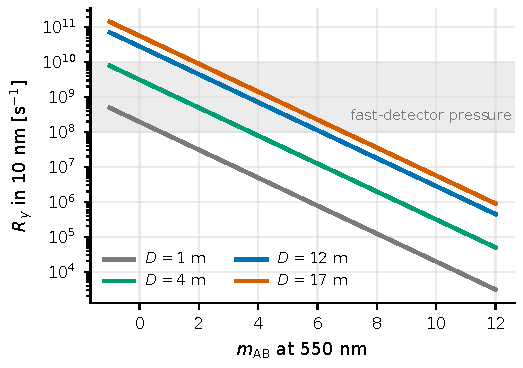
\includegraphics[width=0.86\linewidth]{figures/generated/chapter_18/ch18_photon_rate_magnitude.pdf}
\caption{The conversion from AB magnitude to narrowband photon rate. The curve uses a 550 nm, 10 nm passband and total efficiency $\eta=0.25$. Aperture changes the collecting area only linearly, and each increase of 5 magnitudes drops the photon rate by a factor of 100; the grey region marks the range above $10^8\,{\rm s^{-1}}$, where pressure on high-speed detection and data throughput begins.}
\label{fig:e15-photon-rate}
\end{figure}

\paragraph{Coherence dilution: why the raw photon rate is not the usable signal}

What intensity interferometry truly wants to measure is that tiny bump of the second-order correlation at zero delay, whose height is jointly determined by the optical \textbf{coherence time} $\tau_c$ (Chapter~\ref{chap:e02}) and the electronic response time. The coherence time is "the time the light wave still remembers its own phase," set by the bandwidth: $\tau_c\simeq1/\Delta\nu\simeq\lambda^2/(c\,\Delta\lambda)$. Take the 416 nm, 13 nm passband commonly used by VERITAS:
\[
  \tau_c\simeq\frac{\lambda^2}{c\,\Delta\lambda}
  =\frac{(416\times10^{-7})^2}{3\times10^{10}\times13\times10^{-7}}
  \approx 4.4\times10^{-14}\,{\rm s} .
\]
This is tens of femtoseconds, far faster than any electronics. The equivalent time width of the detector plus electronic chain is $\Delta t\sim4\,{\rm ns}$. The true correlation peak holds only within this narrow time $\tau_c$, yet it is flattened out across the wide time bin $\Delta t$, so the peak height is diluted by about $\tau_c/\Delta t$:
\[
  \frac{\tau_c}{\Delta t}\approx\frac{4.4\times10^{-14}}{4\times10^{-9}}
  \approx1.1\times10^{-5}.
\]
So the normalized correlation peak of unresolved thermal light at zero baseline naturally falls to the order of a few $10^{-6}$: this is precisely the $N_0\sim10^{-6}$ tier measured in the VERITAS papers \citep{2020NatAs...4.1164A,2024ApJ...966...28A}. That the peak is so low means it can only "surface" from the noise by long-time averaging and strict calibration. Figure~\ref{fig:e15-coherence} plots this dilution.

\begin{figure}[tbp]
\centering
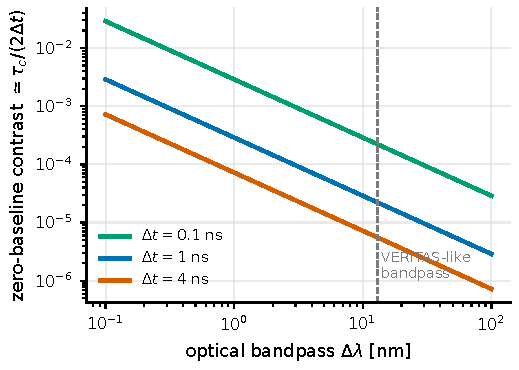
\includegraphics[width=0.86\linewidth]{figures/generated/chapter_18/ch18_coherence_dilution.pdf}
\caption{The wider the passband, the shorter the optical coherence time; the slower the electronic time resolution, the more the zero-delay correlation peak is diluted. The combination of 416 nm, 13 nm, 4 ns gives a contrast of a few $10^{-6}$, so the correlation peak can only appear from the noise by long integration and strict calibration.}
\label{fig:e15-coherence}
\end{figure}

Here lies a counterintuitive but extremely important fact: \textbf{widening the optical passband does not improve the signal-to-noise ratio proportionally}. A wide band does bring more photons ($R_\gamma\propto\Delta\lambda$), but at the same time shortens the coherence time and lowers the correlation contrast in each time bin ($\propto\tau_c\propto1/\Delta\lambda$). The two nearly cancel exactly in the signal-to-noise ratio; the next section will make this evident. A real instrument still has to choose a filter, but that is to control the PMT current, sky background, oblique-incidence effect, or to select spectral lines, not simply "the wider the better" \citep{2020MNRAS.491.1540A,2024MNRAS.529.4387A}.

\section{How to estimate signal-to-noise ratio and integration time}
\label{sec:e15-snr}

With the photon rate, we can ask the question we care about most: how long must one expose for the signal to be strong enough? The intensity-interferometry signal-to-noise scaling derived in Chapter~\ref{chap:e11} is the core of all this:

\begin{equation}
  {\rm SNR}
  = A\,\alpha\,n\,|V(\bm B)|^2\,
    \sqrt{\frac{\Delta f\,T}{2}} .
  \label{eq:e15-snr}
\end{equation}
\begin{formulaexplain}
$A$: the collecting area (${\rm cm^2}$). $\alpha$: the quantum efficiency (dimensionless). $n$: the incident spectral photon density ${\rm photons\,s^{-1}\,cm^{-2}\,Hz^{-1}}$. $|V|^2$: the squared visibility. $\Delta f$: the electronic bandwidth (Hz). $T$: the integration time (s). The signal accumulates as $\sqrt{T}$.
\end{formulaexplain}

First nail down each symbol. $A$ is the effective area of each telescope (${\rm cm^2}$); $\alpha$ is the quantum efficiency (dimensionless); $n$ is the \textbf{incident spectral photon density}, the number of photons per unit area, per unit time, per unit optical bandwidth, with dimensions ${\rm photons\,s^{-1}\,cm^{-2}\,Hz^{-1}}$, determined by the source's surface brightness (i.e. brightness temperature), \emph{independent of how wide an optical passband you choose}. $|V(\bm B)|^2$ is the squared visibility on baseline $\bm B$ (dimensionless, between 0 and 1), the target signal we truly want to measure. $\Delta f$ is the electronic bandwidth (Hz), the equivalent bandwidth jointly determined by the light pulse, PMT/SPAD response, cabling, amplifier, digitizer, and software correlation. $T$ is the integration time (s).

This formula has several things worth chewing over. First, look at $A\,\alpha\,n$ combined: its dimensions are ${\rm s^{-1}\,Hz^{-1}}$, and since ${\rm Hz^{-1}=s}$, the whole is \emph{dimensionless}: it is the mean photon occupation number per mode $\delta=A\alpha n$, i.e. the \textbf{photon degeneracy}. Visible-light thermal stars have $\delta$ of only $10^{-4}$--$10^{-2}$, which is precisely the root of why the intensity-interferometry signal is so faint. Second, because $n$ is a \emph{spectral} density, widening the optical passband does not change $n$: this confirms from the formula the sentence of the previous section, "a wide band does not earn signal-to-noise for free." Third, and most practical: ${\rm SNR}\propto\sqrt{T}$. The signal accumulates not linearly but by the \emph{square root}: to double the signal-to-noise ratio, one must expose for four times as long. This $\sqrt{T}$ law will become the protagonist of the error budget in the next section.

Plug in a real scenario. LeBohec and Holder take $A=100\,{\rm m^2}$, $\alpha=0.3$, $\Delta f=1\,{\rm GHz}$, $T=5\,{\rm h}=1.8\times10^4\,{\rm s}$, $|V|^2=0.5$, and compute that a star of $m_V\simeq6.7$ falls just at the $5\sigma$ tier; under the same conditions a star of $m_V=5$ (1.7 magnitudes brighter, $n$ about 5 times larger) has a signal-to-noise ratio soaring past twenty, while a star of $m_V=9$ has less than $1\sigma$ left, i.e. is unmeasurable \citep{2006ApJ...649..399L,2008AIPC..984..205L}. Plotting this dependence as a magnitude--integration-time heatmap gives Figure~\ref{fig:e15-snr}. Solving conversely for the integration time is also direct: solve Eq.~\eqref{eq:e15-snr} for $T$,
\[
  T = \frac{2\,{\rm SNR}^2}{(A\alpha n)^2\,|V|^4\,\Delta f},
\]
that is, the required time grows with the \emph{square} of the target signal-to-noise ratio, and falls \emph{inversely} with the square of the degeneracy and the fourth power of the visibility, which explains why a fainter target, or one already highly resolved ($|V|^2$ very small), makes the integration time rapidly run out of control.

\begin{figure}[tbp]
\centering
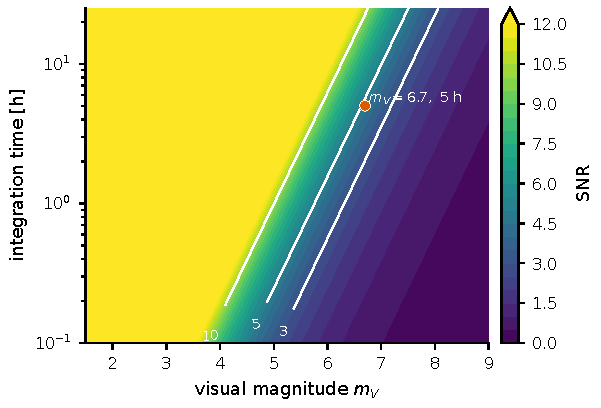
\includegraphics[width=0.90\linewidth]{figures/generated/chapter_18/ch18_snr_heatmap.pdf}
\caption{The dependence of the intensity-interferometry signal-to-noise ratio on magnitude and integration time. The figure takes $A=100\,{\rm m^2}$, $\alpha=0.3$, $\Delta f=1\,{\rm GHz}$, $|V|^2=0.5$; the orange point corresponds to the $m_V\simeq6.7$, 5 h $\approx5\sigma$ position in the LeBohec--Holder estimate.}
\label{fig:e15-snr}
\end{figure}

When using Eq.~\eqref{eq:e15-snr} for a first-round estimate, remember it is the "ideal version." In real data, $T$ is the effective exposure time (live time) after quality slicing, not wall-clock time; $\Delta f$ is the equivalent bandwidth of the whole electronic chain; and $|V|^2$ also varies slowly with the target's altitude and hour angle. Take a set of real engineering numbers: VERITAS uses four 12 m telescopes to give six baselines simultaneously, with a 416 nm, about 13 nm filter and 4 ns sampling, spitting out about 3.5 TB of raw data per hour; MAGIC uses two 17 m telescopes and a central PMT, and its early demonstration reported a sensitivity about an order of magnitude higher than Narrabri. The Vega photon-counting experiment took another route: using a single-photon avalanche diode (SPAD) plus software correlation, it measured $\langle g^{(2)}\rangle=1.0034\pm0.0008$ at zero baseline, while at a projected baseline of about 2 km it showed \emph{no} correlation, exactly as expected since Vega's angular diameter of about 3.3 mas is already fully resolved on that baseline \citep{2020NatAs...4.1164A,2020MNRAS.491.1540A,2021MNRAS.506.1585Z}.

Multiple telescopes buy two things at once: more data and more geometry. $N$ telescopes give $N(N-1)/2$ simultaneous baselines: 4 give only 6, but 60 give 1770. The key is that different baselines sample the source structure at \emph{different points} in the $u,v$ plane, and are by no means repeated measurements of the same number (Chapter~\ref{chap:e11}). To measure the diameter of a uniform disk, a few suitable baselines suffice; but to measure the oblateness of a rapid rotator, a binary, a disk wind, or a non-axisymmetric spectral-line emitting region, position-angle coverage is indispensable. For covering hot-star structures of 0.1--3 mas, the whole baseline range of 30--2000 m is more useful than simply piling up one longest baseline. Figure~\ref{fig:e15-uv} compares the $u,v$ coverage of a small array and a large array.

\begin{figure}[tbp]
\centering
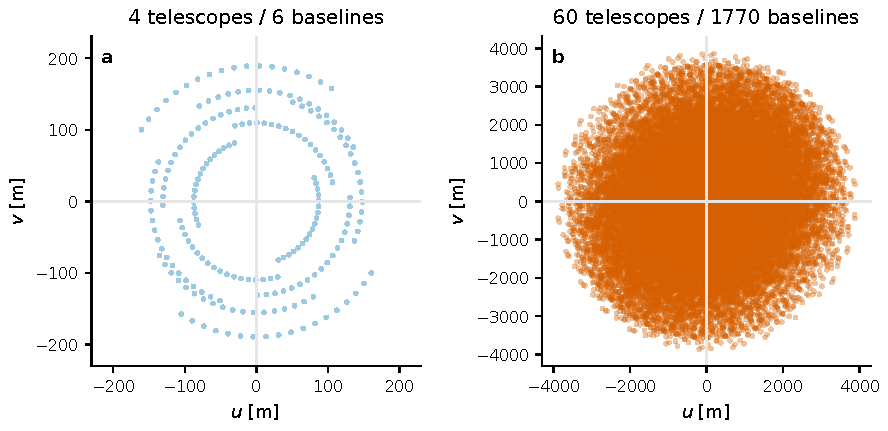
\includegraphics[width=0.94\linewidth]{figures/generated/chapter_18/ch18_uv_coverage.pdf}
\caption{How array size changes $u,v$ sampling. Left: the six baselines of four telescopes, still relatively sparse after rotation with hour angle; right: a multi-telescope array with short, medium, and long baselines present at once. Dense coverage does not automatically mean high signal-to-noise, but it decides whether a non-axisymmetric target can be stably fit or reconstructed.}
\label{fig:e15-uv}
\end{figure}

\section{Baseline, bandwidth, and band choice are decided by the visibility slope}
\label{sec:e15-baseline}

With the signal-to-noise ratio in hand, why can we still not fix the baseline right away? Because \textbf{strong signal} and \textbf{much information} are two different things. A baseline may have a very high correlation peak (very good signal-to-noise), yet be almost insensitive to the angular diameter we want to measure, and then no matter how precisely it measures, it is useless. To judge "which baseline actually carries diameter information," one must look at the \emph{slope} of the visibility curve.

First set out the rough relation between angular scale and baseline. To resolve an angular scale $\theta$, the required baseline is about

\begin{equation}
  B\sim\frac{\lambda}{\theta}
  = 86\,{\rm m}\left(\frac{\lambda}{416\,{\rm nm}}\right)
                \left(\frac{1\,{\rm mas}}{\theta}\right).
  \label{eq:e15-baseline}
\end{equation}
\begin{formulaexplain}
$B$: the required baseline (m). $\lambda$: the observing wavelength. $\theta$: the target angular scale (here in mas). This is an order-of-magnitude formula: to resolve a smaller angle, a longer baseline is needed; the shorter the wavelength, the finer the same baseline resolves.
\end{formulaexplain}

Plug in a few numbers for a picture: a $\theta=2\,{\rm mas}$ hot star at 416 nm begins to be resolved at only about 43 m; $\theta=0.5\,{\rm mas}$ needs about 170 m; $\theta=0.1\,{\rm mas}$ requires reaching about 860 m. Narrabri's maximum baseline is about 188 m, so it is best at bright, hot stars with angular diameters from a few tenths to a few mas; a CTA-class kilometre array can push the spatial frequency to tens of microarcseconds, but the target must still have enough photon rate to afford it \citep{1974MNRAS.167..121H,2006ApJ...649..399L}.

Now look at the slope. The squared visibility of a uniform disk (Chapter~\ref{chap:e11}) is first a plateau near 1 with baseline, then decreases, hitting bottom at the first zero. The crux of observation design is: if all your baselines fall on the $|V|^2\simeq1$ plateau, the curves for different $\theta$ nearly coincide and you cannot tell the star's size at all; if you only measure the extremely low visibility \emph{after} the first zero, the correlation peak is so low it hugs the noise. \textbf{Diameter information is concentrated on the section of the baseline where the curve drops most steeply, i.e. where the slope $|\partial|V|^2/\partial\theta|$ is largest}, usually in the descending region of the first lobe and near the first zero. So a serious feasibility calculation must not only plot the target model's $|V|^2(B)$, but also its derivative with respect to the parameter, $\partial|V|^2/\partial\theta$, to see which baseline the peak falls on (Figure~\ref{fig:e15-vis}).

\begin{figure}[tbp]
\centering
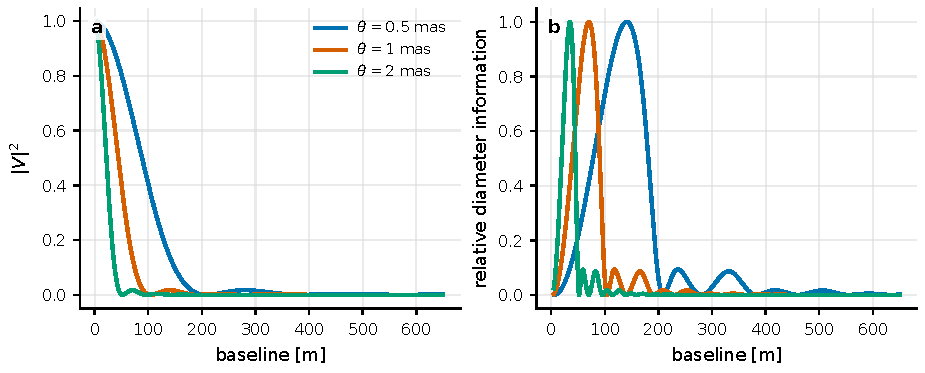
\includegraphics[width=0.94\linewidth]{figures/generated/chapter_18/ch18_visibility_fisher.pdf}
\caption{The squared visibility curve of a uniform disk and its diameter sensitivity. At 416 nm, the descending regions of 2 mas, 1 mas, and 0.5 mas targets fall on baselines of tens of metres, a hundred metres, and a few hundred metres respectively; the right panel shows that diameter information comes mainly from baselines with large curve slope, while the short-baseline plateau $|V|^2\simeq1$ is almost insensitive to the diameter.}
\label{fig:e15-vis}
\end{figure}

Writing this intuition as a formula is the Fisher information of Chapter~\ref{chap:e12}. For a single parameter $\theta$ and a set of independent baseline measurements $\mu_i=|V_i|^2$, the Fisher information and the attainable variance are

\begin{equation}
  I(\theta)=\sum_i
  \frac{1}{\sigma_i^2}
  \left(\frac{\partial\mu_i}{\partial\theta}\right)^{\!2},
  \qquad
  \sigma_\theta\ge\frac{1}{\sqrt{I(\theta)}} .
  \label{eq:e15-fisher}
\end{equation}
\begin{formulaexplain}
$\mu_i$: the observable on the $i$-th baseline (such as $|V_i|^2$). $\partial\mu_i/\partial\theta$: its sensitivity (slope) to the target parameter. $\sigma_i$: the error of that measurement. The right side is the Cramér--Rao lower bound. Baselines with large slope and small error contribute the most.
\end{formulaexplain}

This formula turns the preceding sentences into a computable criterion. Each baseline's contribution is \emph{slope squared divided by error squared}: a large slope $\partial\mu_i/\partial\theta$ and a small error $\sigma_i$ contribute much. So two kinds of "seemingly fine but useless" baselines are immediately exposed: a baseline with a very small error but near-zero slope (on the plateau) contributes almost nothing; a baseline with a very large slope but $|V|^2$ so low that the correlation peak is buried in noise, giving a huge $\sigma_i$, also cannot hold up the result. Note that $\sigma_i$ must include both the statistical noise (from Eq.~\eqref{eq:e15-snr}) and the systematic terms of the next section. The VERITAS observation of the rapid rotator $\gamma$ Cas is a living example: different projected baselines sample $|V|^2$ in different directions, and only then can the oblateness and long-axis direction be constrained; a single equivalent circular-disk diameter simply cannot describe such a non-axisymmetric target \citep{2025ApJ...995..191A,2024ApJ...966...28A}.

Band choice is decided along with it. The same physical baseline samples a spatial frequency about 1.9 times higher at 416 nm than at 800 nm: the blue end has higher resolution, but atmospheric transmission, mirror reflectivity, detector quantum efficiency, and oblique filter incidence are all harder to deal with. Spectral-line observations require a different ledger: one computes the line flux rather than the broadband magnitude. For hot stars and Be stars, H$\alpha$, helium lines, or metal lines may come from an emitting region larger than the continuum; using narrowband to separate the geometric structure and the velocity channels is worthwhile, but the event rate, filter leakage, and background of each channel must all be recomputed \citep{2012NewAR..56..143D,2021MNRAS.506.1585Z}.

\section{Error budget: the statistical floor and the systematic floor}
\label{sec:e15-error-budget}

Now we come to the most practical, and most often overlooked by outsiders, section of the whole chapter. A novice writing an observing proposal often reports only a signal-to-noise ratio and is done. But the signal-to-noise ratio governs only the \emph{statistical} noise, which falls all the way with integration time; what truly decides "how precisely you can actually measure" is often a layer of \textbf{systematic floor that does not fall with time}. Separating the two is the error budget.

For one parameter $\theta$ to be fit, add the various errors in quadrature:

\begin{equation}
  \sigma_\theta^2
  = \sigma_{\rm stat}^2
  + \sigma_{\rm bg}^2
  + \sigma_{\rm time}^2
  + \sigma_{\rm cal}^2
  + \sigma_{\rm model}^2 .
  \label{eq:e15-error-budget}
\end{equation}
\begin{formulaexplain}
$\sigma_\theta$: the total error of the target parameter. The right side is, in order, the statistical, background, time, calibration, and model error. When independent, they add in quadrature. This formula reminds you: reporting one signal-to-noise ratio is not enough; you must also say clearly where the error floor comes from.
\end{formulaexplain}

Spell out each term: what it is, with dimensions all converted to the units of $\theta$. $\sigma_{\rm stat}$ comes from the finite coincidence count or correlation-peak fit, the direct consequence of the signal-to-noise ratio of Eq.~\eqref{eq:e15-snr}. $\sigma_{\rm bg}$ comes from the uncertainty of the off-source interpolation and the dark current. $\sigma_{\rm time}$ comes from the clock, geometric delay, sampling, and peak shape. $\sigma_{\rm cal}$ comes from the calibrator star, the total system transmission, the filter, and polarization. $\sigma_{\rm model}$ comes from the source model itself: forcing a rapid rotator into a disk, forcing a spectral-line disk into a Gaussian, or ignoring a companion star all introduce this term.

The key physics is that they \emph{behave differently with time}. The statistical term obeys the shot-noise $\sqrt N$ law (Chapter~\ref{chap:e03}): the count $N\propto T$, so

\begin{equation}
  \sigma_{\rm stat}(T)=\frac{c_0}{\sqrt{T}} ,
  \qquad
  \sigma_{\rm sys}^2=\sigma_{\rm bg}^2+\sigma_{\rm time}^2
        +\sigma_{\rm cal}^2+\sigma_{\rm model}^2 ,
  \label{eq:e15-floor}
\end{equation}
\begin{formulaexplain}
$c_0$: a constant determined by the photon rate, visibility slope, etc. $\sigma_{\rm stat}\propto T^{-1/2}$ falls with exposure; $\sigma_{\rm sys}$ gathers the systematic terms that do not fall with time. The total error is the quadrature sum of the two.
\end{formulaexplain}

Here $c_0$ is a constant absorbing the photon rate, visibility slope, and calibration chain (with units consistent with $\theta$). The picture is clear: $\sigma_{\rm stat}$ is like a continuously sliding slope, lower the longer you expose; while $\sigma_{\rm sys}$ is a \emph{horizontal floor}. The total error is the quadrature sum of the two, initially dominated by the statistical slope and falling with $T$, until it hits the systematic floor and \emph{stops moving}. The moment of hitting is when the statistical term equals the systematic term:
\[
  \sigma_{\rm stat}(T_\star)=\sigma_{\rm sys}
  \;\Longrightarrow\;
  T_\star=\left(\frac{c_0}{\sigma_{\rm sys}}\right)^{2}.
\]
\textbf{Adding time beyond $T_\star$ is almost wasted}: the total error already hugs the systematic floor, and quadrupling $T$ again only halves the statistical term, which is already far below the floor and has no effect on the total error. This is the sentence that should be made clearest, and most written into a proposal, in a feasibility calculation: not "the longer the exposure the better," but "one should stop when the statistical term falls near the systematic floor, and the remaining precision must be won by lowering the systematic terms." Figure~\ref{fig:e15-budget} plots this behaviour of the slope hitting the floor.

\begin{figure}[tbp]
\centering
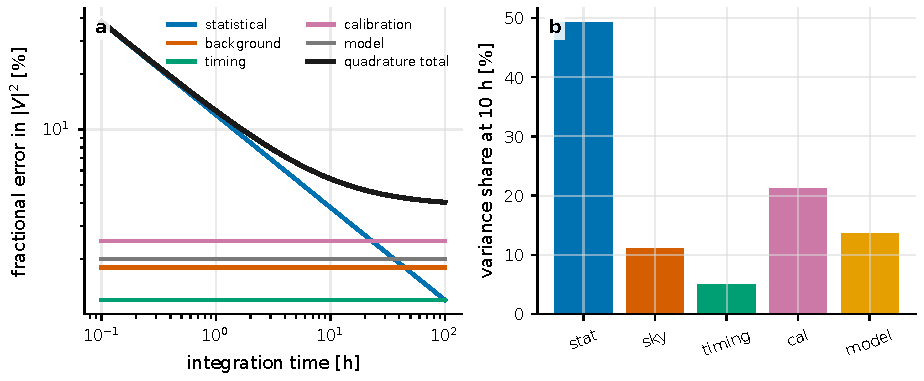
\includegraphics[width=0.94\linewidth]{figures/generated/chapter_18/ch18_error_budget.pdf}
\caption{The statistical and systematic terms in the error budget. Left: the statistical error falls with integration time, but the background, time, calibration, and model terms combine into a plateau; right: the contribution of each term to the total variance at 10 h. An observing proposal should connect every term to an observable calibration dataset, and give the error plateau in addition to the total signal-to-noise ratio.}
\label{fig:e15-budget}
\end{figure}

The most common and most easily quantified systematic term is \textbf{background dilution}. If there is, outside the source, a background light \emph{uncorrelated} with the signal (skyglow, moonlight, dark counts), it does not create a false correlation but proportionally lowers the true correlation peak. Let the ratio of background to starlight at one end be $\beta$; when symmetric at both ends, the observed contrast shrinks by $(1+\beta)^{-2}$ (Chapter~\ref{chap:e08}). Plug in numbers: at $\beta=0.03$ (background only 3\% of starlight), $(1.03)^{-2}=0.94$, only a 6\% drop, almost harmless; but at $\beta=0.5$, $(1.5)^{-2}=0.44$, the peak has only about forty percent left. The VERITAS analysis of $\beta$ UMa used off-source observations (off runs) about $0.5^\circ$ from the target to estimate the non-stellar-light current, with a typical off-source intensity only about 3\% of that on source, so the effect on the radius fit is small; but once there is a bright moon, cloud, fog, city light, or detector afterpulsing, this approximation worsens and separate quality slicing is required \citep{2024ApJ...966...28A,2025ApJ...995..191A}. Figure~\ref{fig:e15-bg} gives the dilution factor and its inverse correction.

\begin{figure}[tbp]
\centering
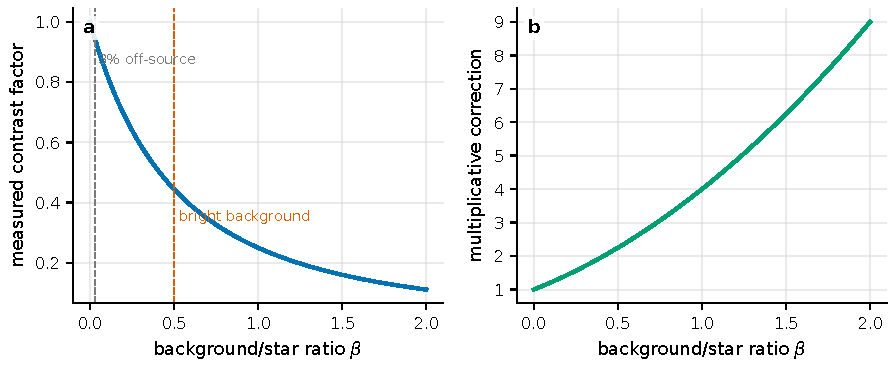
\includegraphics[width=0.94\linewidth]{figures/generated/chapter_18/ch18_background_dilution.pdf}
\caption{The dilution of the correlation peak by uncorrelated background. When the background/starlight ratio is the same at both ends, the observed contrast falls by $(1+\beta)^{-2}$: $\beta=0.03$ causes only a few percent correction, while $\beta=0.5$ has already pressed the peak to about 44\%. The right panel is the inverse correction factor; the larger the correction, the more sensitive it is to the background-estimate error.}
\label{fig:e15-bg}
\end{figure}

Time calibration is a hard boundary common to both intensity interferometry and photon counting. The correlation peak width is usually a few nanoseconds; if the relative delay model of the two telescopes is wrong by 1 ns, the peak is smeared wide, or even moved out of the fitting window. In the Vega photon-counting experiment, the relative time precision of the zero-baseline sub-apertures was about 100 ps, and between the two telescopes one still had to handle the light-travel time, instrument delay, GPS or rubidium clock drift, and fibre dispersion, finally correlating with a time bin of about 400 ps; they explicitly pointed out that a multi-telescope scheme must achieve about nanosecond-scale synchronization to keep the observation time at the hour scale. VERITAS uses White Rabbit's 10 MHz clock distribution plus 4 ns sampling, yet must still track the drift of the optical-path delay with hour angle within each run, and handle the run-to-run peak-position variation \citep{2021MNRAS.506.1585Z,2024ApJ...966...28A}.

The calibrator star must be chosen as carefully as the science target. An ideal calibrator should have a known angular diameter, stable luminosity, a sky position close to the target, a similar colour, and a sufficiently high photon rate. If the target is a 0.5 mas hot star, and the calibrator's own diameter has a 5\% uncertainty, then the final diameter error is easily dominated by this term $\sigma_{\rm cal}$, and exposing longer is of no use. Modern intensity-interferometry observations often first take a hot star of known angular diameter as a reference, check the zero-baseline normalization, filter response, and $|V|^2(B)$ shape, and then measure the unknown target. MAGIC's 2024 performance paper used several reference stars to validate the system and then gave new stellar angular diameters; VERITAS went from the disk diameter of $\beta$ UMa all the way to the oblateness and position angle of $\gamma$ Cas, using the same calibration framework \citep{2024MNRAS.529.4387A,2024ApJ...966...28A,2025ApJ...995..191A}.

\section{A feasibility calculation from beginning to end}
\label{sec:e15-worked}

Now let us string the whole chapter into one real calculation. Let the science goal be: \textbf{use a VERITAS-type array to measure the angular diameter of a hot, bright star, pressing the relative error to a few percent}. The array parameters are all taken from the real VERITAS intensity-interferometry system; the target is a hot star sitting at the edge of sensitivity, so that this problem is neither "easily measurable" nor "hopeless."

\textbf{Step 0: write down the target parameters and success criteria.} The physical quantity to measure is the angular diameter $\theta$, with target precision $\sigma_\theta/\theta\lesssim3\%$. The success criteria are quantified as: at least three baselines reach ${\rm SNR}>5$ in the descending region of the first lobe; the normalization drift of the repeated calibrator observations is less than 3\%; and the off-source background correction is less than 10\% of the total signal.

\textbf{Step 1: choose the target, fix the photon rate.} We deliberately pick a hypothetical early-type star at $m_V\approx5$ with effective temperature about $10^4\,{\rm K}$, fainter than VERITAS's real bright targets such as $\beta$ UMa ($m_V\approx2.4$) and $\gamma$ Cas ($m_V\approx2.2$) and sitting right at the edge of sensitivity, so that the problem is not too easy. (A reminder: the $m_V\approx5$, $T_{\rm eff}\approx10^4\,{\rm K}$, $\theta\approx0.7\,{\rm mas}$ used in this section are illustrative numbers given \emph{independently} to demonstrate each step, and need not correspond to the same real star: if one seriously plugs them into the Stefan--Boltzmann relation $f_{\rm bol}=\sigma T^4(\theta/2)^2$, one finds these three numbers are not strictly self-consistent, and the reader need not dwell on this.) Using the chain of Section~\ref{sec:e15-photon-budget}, a 12 m telescope at 550 nm, 10 nm passband, $\eta=0.25$ gives $R_\gamma\simeq2.8\times10^8\,{\rm s^{-1}}$. Switching to VERITAS's actual 416 nm, 13 nm filter, the photon rate is of the same order. Conclusion: photons are plentiful, and this star will not drop out for being too faint.

\textbf{Step 2: estimate the angular scale, fix the baseline.} A $10^4\,{\rm K}$ early-type bright star usually has an angular diameter of 0.5--1 mas. By Eq.~\eqref{eq:e15-baseline}, a star of $\theta\approx0.7\,{\rm mas}$ at 416 nm has its first-lobe descending region falling around $86/0.7\approx120\,{\rm m}$. VERITAS's six baselines from four 12 m telescopes cover tens of metres to about 170 m, exactly bracketing the descending region and near the first zero: this means we have several baselines falling where the \emph{slope is large}, satisfying the diameter-information criterion of Section~\ref{sec:e15-baseline}.

\textbf{Step 3: estimate the correlation-peak height and the statistical signal-to-noise ratio.} By Section~\ref{sec:e15-photon-budget}, 416 nm, 13 nm, 4 ns give $\tau_c\simeq4.4\times10^{-14}\,{\rm s}$, and the diluted zero-baseline peak is about a few $10^{-6}$. Substituting the array parameters into Eq.~\eqref{eq:e15-snr}: the equivalent LeBohec--Holder calculation shows that with $A=100\,{\rm m^2}$, $\alpha=0.3$, $\Delta f=1\,{\rm GHz}$, $|V|^2=0.5$, a star of $m_V\simeq6.7$ reaches $5\sigma$ in 5 h; our star at $m_V\approx5$ is about 5 times brighter, so the same 5 h single-baseline signal-to-noise ratio can soar past twenty. Taking a conservative single-baseline ${\rm SNR}\approx5$--$10$ is already sufficient.

\textbf{Step 4: translate the signal-to-noise ratio into the angular-diameter error.} The relative error of the correlation peak is $\sigma_{|V|^2}/|V|^2\approx1/{\rm SNR}$. To convert it into the angular-diameter error, use one \textbf{error propagation}: the observable $|V|^2$ is a function of $\theta$, and a small error in $\theta$ is carried by the derivative into an error in $|V|^2$,
\[
  \sigma_{|V|^2}=\left|\frac{\partial|V|^2}{\partial\theta}\right|\,\sigma_\theta .
\]
Dividing both sides by $|V|^2$ and $\theta$, the right side neatly assembles into the logarithmic derivative $\partial\ln|V|^2/\partial\ln\theta=(\theta/|V|^2)\,\partial|V|^2/\partial\theta$, so
\[
  \frac{\sigma_\theta}{\theta}
  =\frac{\sigma_{|V|^2}/|V|^2}{\left|\partial\ln|V|^2/\partial\ln\theta\right|} .
\]
In the descending region, the \emph{logarithmic slope} of the visibility with respect to the diameter $|\partial\ln|V|^2/\partial\ln\theta|$ is of order 1--2; substituting $\sigma_{|V|^2}/|V|^2\approx1/{\rm SNR}$ gives
\[
  \frac{\sigma_\theta}{\theta}
  \approx\frac{1}{{\rm SNR}}\,
  \frac{1}{\left|\partial\ln|V|^2/\partial\ln\theta\right|}
  \approx\frac{1}{5}\times\frac{1}{1.5}
  \approx13\%
\]
That is, a \emph{single} large-slope baseline gives about a dozen percent in 5 h. Then use Eq.~\eqref{eq:e15-fisher} to add the information of multiple baselines: $N_b$ equally useful baselines shrink the statistical error by $1/\sqrt{N_b}$, and if three of the six baselines fall in the descending region, $\sigma_\theta/\theta$ is pressed to about $13\%/\sqrt3\approx7\%$; adding a few more nights, or the more baselines of more telescopes, makes reaching 3\% realistic. This step turns "signal-to-noise ratio" genuinely into "to what fraction of a percent the angular diameter can be measured."

\textbf{Step 5: check the error budget, decide whether to keep exposing.} Use Eq.~\eqref{eq:e15-error-budget} and \eqref{eq:e15-floor} to check the systematic floor. Background: off-source $\beta\approx0.03$, a dilution correction of about 6\%, calibratable by off-source observations, so $\sigma_{\rm bg}$ is small. Time: White Rabbit plus 4 ns sampling, relative delay controlled at the nanosecond scale, so $\sigma_{\rm time}$ is manageable. Calibration: if the calibrator's diameter is known to 3\%, then $\sigma_{\rm cal}$ is about 3\%, which is exactly of the same order as our target precision, becoming the \textbf{most likely systematic floor}. By Eq.~\eqref{eq:e15-floor}, when the statistical term $\sigma_{\rm stat}$ is exposed down to about 3\% (corresponding to $T_\star$), the total error hugs this floor set by the calibrator, and \emph{adding more exposure is meaningless}. The conclusion is plain: whether this observation can reach 3\% depends in the end not on exposing a few more hours, but on \emph{whether there is a calibrator with a sufficiently well-determined diameter}.

\textbf{Step 6: write it into the feasibility conclusion of the proposal.} One sentence to close: for a hot star of $m_V\approx5$, $\theta\approx0.7\,{\rm mas}$, using VERITAS's six baselines, 416 nm/13 nm, 4 ns sampling, several nights of effective exposure can reach ${\rm SNR}>5$ on multiple baselines in the descending region, pressing the angular-diameter statistical error to about 3\%; the systematic floor is dominated by the calibrator's diameter uncertainty (about 3\%), so the upgrade direction is not longer exposure, but a better calibrator and stricter filter/background control. If no correlation is detected on the longest baseline, one can still give an \emph{upper limit} on the angular diameter or rule out an emitting region too large: returning empty-handed is also a valuable result.

This estimation chain is not exclusive to intensity interferometry. Amplitude interferometry, the quantum-network telescope, CMB polarization, and the photon statistics of fast radio bursts (FRBs), down to a laboratory teaching bench, all use the same skeleton: event rate $\to$ number of modes $\to$ response function $\to$ calibration terms $\to$ model derivatives $\to$ error budget; the difference is only in the specific form of the observable $\mu_i$. The ranking of science cases should also follow this line of thought, scoring "scientific value" and "observability" separately in two columns, and not conflating a \emph{beautiful} target with a \emph{doable} one \citep{2010SPIE.7734E..0AD,2012MNRAS.419..172N,2013APh....43..331D,2022SPIE12183E..0DK}. Table~\ref{tab:e15-checklist} lists the common ranges and uses of each quantity in this ledger as a checklist.

\begin{longtable}{p{0.16\linewidth}p{0.30\linewidth}p{0.44\linewidth}}
\caption{Feasibility-ledger quick-reference table: the common range and planning use of each quantity.}
\label{tab:e15-checklist}\\
\toprule
Quantity & Common range & Use in the plan \\
\midrule
\endfirsthead
\toprule
Quantity & Common range & Use in the plan \\
\midrule
\endhead
$m_V,\,m_B$ & $-1$ to $9$ mag, the current main battleground of intensity interferometry & Convert to $R_\gamma$ via Eqs.~\eqref{eq:e15-ab-flux} and \eqref{eq:e15-photon-rate}, first judging whether the target is too faint. \\
$A_{\rm eff}$ & $1$--$250\,{\rm m^2}$ per telescope & Enters the photon rate and signal-to-noise ratio; mirror ageing, obscuration, and fibre coupling must all be folded into the efficiency. \\
$\Delta\lambda$ & $0.1$--$30\,{\rm nm}$ & Determines the coherence time, PMT current, sky background, and spectral-line selection. \\
$\Delta t$ & $0.1$--$5\,{\rm ns}$ & Determines the degree of correlation-peak dilution and the usable electronic bandwidth. \\
$B_p$ & $10$--$2000\,{\rm m}$ & Determines the angular scale and $u,v$ coverage; short and long baselines constrain different structures. \\
$\beta$ & $0.01$--$1$ & The background/starlight ratio, determining the contrast dilution and the background systematic error. \\
$\sigma_{\rm cal}$ & $1\%$--$10\%$ of the visibility or diameter & Often becomes the error floor after long exposure. \\
\bottomrule
\end{longtable}

\section{Chapter Summary}
\label{sec:e15-summary}

\begin{itemize}
  \item \textbf{An observation is a ledger.} Eq.~\eqref{eq:e15-likelihood} connects the physical parameters to the data via "instrument observable + calibration + background"; designing an observation is computing this chain segment by segment into real numbers, not merely writing "which star to look at." The event table is the raw broth, the image is the boiled-down spoonful: information averaged away at recording cannot be recovered.
  \item \textbf{The photon budget has four steps.} Magnitude $\to$ spectral flux density (Eq.~\eqref{eq:e15-ab-flux}) $\to$ photon flux per unit area $\to$ multiply by area and efficiency to get the effective photon rate (Eq.~\eqref{eq:e15-photon-rate}). A 12 m telescope gives $R_\gamma\simeq2.8\times10^8\,{\rm s^{-1}}$ for an $m_{\rm AB}=5$ star; but coherence dilution $\tau_c/\Delta t\sim10^{-5}$ presses the zero-baseline peak to a few $10^{-6}$.
  \item \textbf{Signal-to-noise accumulates as $\sqrt T$.} In Eq.~\eqref{eq:e15-snr}, ${\rm SNR}\propto A\alpha n|V|^2\sqrt{\Delta f\,T}$; $A\alpha n$ is the photon degeneracy $\delta\sim10^{-4}$--$10^{-2}$. Because $n$ is a spectral density, widening the optical passband earns almost no free signal-to-noise. To double the precision, one must expose four times as long.
  \item \textbf{The baseline is chosen by the visibility slope.} Diameter information is concentrated in the descending region where $|\partial|V|^2/\partial\theta|$ is largest (Eq.~\eqref{eq:e15-fisher}); a baseline on the plateau with near-zero slope contributes nothing however small its error, and a baseline with $|V|^2$ too low is buried in noise however large its slope.
  \item \textbf{Error budget $=$ statistical floor $+$ systematic floor.} Eqs.~\eqref{eq:e15-error-budget} and \eqref{eq:e15-floor}: $\sigma_{\rm stat}\propto T^{-1/2}$ slides all the way down, while the systematic terms (background, time, calibration, model) are a horizontal floor. After exposing to $T_\star=(c_0/\sigma_{\rm sys})^2$, once the statistical term hits the floor, \emph{adding more exposure is meaningless}: the remaining precision must be won by lowering the systematic terms.
  \item \textbf{The feasibility calculation has a fixed routine.} Target parameters $\to$ photon rate $\to$ baseline $\to$ signal-to-noise ratio $\to$ angular-diameter error $\to$ error-budget stopping decision. This skeleton applies equally to amplitude interferometry, the quantum-network telescope, CMB polarization, and FRB photon statistics, with the difference only in the form of the observable.
\end{itemize}

\medskip
\noindent\textbf{Questions to Ponder.}
(1) If the optical passband is widened from 10 nm to 30 nm, the photon rate rises 3 times, yet the intensity-interferometry signal-to-noise ratio barely moves: explain why using the fact that $n$ in Eq.~\eqref{eq:e15-snr} is a spectral density.
(2) You have exposed for 5 h with a statistical error of 4\%, but the calibrator diameter is known only to 3\%. Is it worth exposing to 20 h? Use Eq.~\eqref{eq:e15-floor} to compute from what to what the total error would fall.
(3) A star's angular diameter is estimated at 0.3 mas, and the longest baseline you have is only 100 m (416 nm). Which section of the visibility curve do you fall on? Is this baseline sensitive to the diameter? Should you seek a longer or a shorter baseline?
